%%%%%%%%%%%%%%%%%%%%%%%%%%%%%%%%%%%%%%%%%
% TMDEI Dissertation
% LaTeX Template
% Version 0.1 (Dec/2015)
%
% Adapted to TMDEI/ISEP style (Dec/2015) by
%  Nuno Pereira (nap@isep.ipp.pt) and
%  Paulo Baltarejo (pbs@isep.ipp.pt)
%
% Based on MastersDoctoralThesis Version 1.2 by Vel (vel@latextemplates.com) and
% Johannes Böttcher, downloaded from (21/11/15):
% http://www.LaTeXTemplates.com
%
% This template is originally based on a template by:
% Steve Gunn (http://users.ecs.soton.ac.uk/srg/softwaretools/document/templates/)
% Sunil Patel (http://www.sunilpatel.co.uk/thesis-template/)
%
% Template license:
% CC BY-NC-SA 3.0 (http://creativecommons.org/licenses/by-nc-sa/3.0/)
%
%%%%%%%%%%%%%%%%%%%%%%%%%%%%%%%%%%%%%%%%%
%----------------------------------------------------------------------------------------
%	PACKAGES AND OTHER DOCUMENT CONFIGURATIONS
%----------------------------------------------------------------------------------------

\documentclass[
11pt,
portuguese,
singlespacing,
liststotoc,
parskip,
nohyperreflinkcolor,
headsepline,
]{tmdei-style}

\usepackage{amsmath}
\usepackage{tabularx}
\usepackage{tikz}
\usetikzlibrary{positioning,arrows.meta,shapes.geometric,decorations.pathreplacing}

\usepackage[hidelinks]{hyperref}

\usepackage[style=authoryear-comp,backend=biber,uniquename=false]{biblatex}
\addbibresource{mainbibliography.bib}

\makeglossaries

%----------------------------------------------------------------------------------------
%	THESIS INFORMATION
%----------------------------------------------------------------------------------------

\thesistitle{Agentes baseados em LLM com supervisão humana para automação de processos internos de I\&D em saúde digital}

\author{Luís \textsc{Santos}}

\subjectarea{Software Engineering}

\coverprogram{Mestrado em Engenharia de Software} % Texto no cabeçalho da capa

\advisor{Prof. Dra. Elsa Maria De Carvalho Ferreira \textsc{Gomes}}

%\advisors{...} % \advisors has a bug in the cls (\def\advplural without {}), use \advisor instead

\coadvisor{Prof. Diogo Marcelo Esterlita \textsc{Nogueira}}

\supervisor{Cláudia \textsc{Dias} e Daniel \textsc{Rodrigues}} % Company supervisors (VirtualCare). \supervisors has a bug in the cls (\def\supplural without {}), use \supervisor instead

%\cosupervisor{...} % Co-supervisor: not applicable

% if committeepresident is defined, will add the thesis committee to the front page
%\committeepresident{...} % To be filled after jury assignment

%\committeemembers{...} % To be filled after jury assignment

\keywords{LLM Agents, Human-in-the-Loop, Process Automation, Retrieval-Augmented Generation, Digital Health, Audit Trail} % Up to 6 keywords

\university{\href{https://www.isep.ipp.pt}{Instituto Superior de Engenharia do Porto}}

\department{\href{https://www.dei.isep.ipp.pt}{Departamento de Engenharia Informática}}

\thesisdate{Porto, \today}

\hypersetup{pdftitle=\ttitle}
\hypersetup{pdfauthor=\authorname}
\hypersetup{pdfkeywords=\keywordnames}

\begin{document}

%----------------------------------------------------------------------------------------
%	FRONT MATTER
%----------------------------------------------------------------------------------------

%All acronyms must be written in this file.


\frontmatter % Use roman page numbering style (i, ii, iii, iv...) for the pre-content pages

\pagestyle{plain} % Default to the plain heading style until the thesis style is called for the body content

%----------------------------------------------------------------------------------------
%	COVER PAGE
%----------------------------------------------------------------------------------------

\makecoverpage

%----------------------------------------------------------------------------------------
%	TITLE PAGE
%----------------------------------------------------------------------------------------

\maketitlepage


%----------------------------------------------------------------------------------------
%	STATEMENT of INTEGRITY
%----------------------------------------------------------------------------------------
\integritystatement

%----------------------------------------------------------------------------------------
%	ABSTRACT PAGE
%----------------------------------------------------------------------------------------

\begin{abstract}
% Resumo alargado em português (~1000 palavras) — obrigatório para dissertações escritas em inglês.

As organizações de saúde digital realizam frequentemente tarefas manuais e repetitivas no âmbito dos seus processos internos de investigação e desenvolvimento (I\&D), tais como a documentação de projetos, a organização de espaços de trabalho e a geração de secções recorrentes em relatórios. Estas tarefas consomem tempo significativo às equipas, limitando a capacidade de se concentrarem em trabalho de maior valor acrescentado.

Os avanços recentes em modelos de linguagem de grande escala (LLM — \textit{Large Language Models}) e nas arquiteturas de agentes inteligentes abrem novas possibilidades para automatizar este tipo de fluxos de trabalho. Em particular, a combinação de agentes LLM com ferramentas externas e com Geração Aumentada por Recuperação (RAG — \textit{Retrieval-Augmented Generation}) permite criar sistemas capazes de aceder a informação contextual, executar ações sobre sistemas externos e gerar conteúdo fundamentado em documentação existente.

No entanto, o domínio da saúde impõe restrições específicas que tornam a automação direta inviável sem salvaguardas adequadas. Entre os principais riscos destacam-se as alucinações dos modelos, a execução de ações irreversíveis sem validação humana, e as obrigações de rastreabilidade e privacidade decorrentes do Regulamento Geral sobre a Proteção de Dados (RGPD) e do Regulamento Europeu de Inteligência Artificial (AI Act). A literatura existente sobre autonomia humano-máquina (Parasuraman et al., 2000; Shneiderman, 2020) fornece modelos conceptuais úteis, mas é escassa em orientações práticas sobre como operacionalizar estes princípios em contextos reais de I\&D.

Esta dissertação responde à seguinte pergunta central: \textit{como conceber agentes LLM que automatizem processos internos de I\&D em saúde digital, mantendo supervisão humana e rastreabilidade, com ganhos mensuráveis de eficiência sem perda de qualidade nem de confiança por parte da equipa?} Como questão secundária, avalia-se o impacto na eficiência, na qualidade dos outputs e na aceitação dos utilizadores.

O trabalho é desenvolvido no contexto da VirtualCare, empresa portuguesa de saúde digital, onde são identificados dois a três processos de I\&D representativos. Para cada processo selecionado, é definido um modelo de autonomia que classifica cada ação possível do agente em três categorias: ações autónomas (executadas sem intervenção humana), ações sujeitas a aprovação (o agente propõe, o humano valida) e ações proibidas (nunca executadas de forma autónoma). Este modelo operacionaliza o conceito de \textit{Human-in-the-Loop} (HITL), garantindo que a supervisão humana ocorre precisamente nos pontos críticos de cada fluxo.

A metodologia adotada é a \textit{Design Science Research} (Hevner et al., 2004; Peffers et al., 2007), que enquadra o trabalho como a conceção e avaliação de um artefacto (o protótipo dos agentes) em resposta a um problema prático. O processo inclui: levantamento por entrevistas junto da equipa da VirtualCare para mapeamento dos processos; desenho do modelo de autonomia e da arquitetura dos agentes; implementação de um protótipo funcional para dois processos; e ensaios comparativos com a equipa.

O protótipo é avaliado segundo critérios quantitativos e qualitativos. Em termos de eficiência, é estabelecida uma meta de redução mínima de 30\% do tempo face ao processo manual. A qualidade dos outputs é medida por correção e completude (meta: $\geq$85\%) e por capacidade de deteção de erros injetados (meta: $\geq$80\%). A aceitação dos utilizadores é avaliada através do \textit{System Usability Scale} (SUS, Brooke, 1996), com limiar de 68, e de uma escala de utilidade percebida com meta $\geq$4/5.

São comparadas pelo menos três configurações: um fluxo fixo baseado em prompts sem autonomia do agente, um agente com ferramentas e RAG com nível de autonomia máxima, e variantes intermédias com diferentes níveis de supervisão humana. O baseline é o processo manual existente na VirtualCare.

A rastreabilidade é assegurada através de registos de auditoria que cobrem 100\% das ações do agente, sem exceções. Nenhuma ação irreversível é executada sem aprovação prévia de um utilizador humano. Os dados utilizados nos ensaios são anonimizados ou sintéticos, de acordo com as restrições de confidencialidade aplicáveis.

O trabalho contribui com orientações práticas e replicáveis para a integração de agentes LLM em fluxos de trabalho organizacionais sensíveis, com supervisão humana adequada. Estas orientações são concebidas de forma a serem generalizáveis a outros contextos de saúde digital com características semelhantes.

% TODO: expandir para ~1000 palavras com detalhes da implementação e resultados (a preencher no 2.º semestre)

\end{abstract}

\begin{abstractotherlanguage}

Organisations in digital health routinely perform time-consuming manual tasks as part of their research and development (R\&D) processes — including project documentation, workspace organisation, and the generation of recurring report sections. Large Language Model (LLM) agents equipped with tools and Retrieval-Augmented Generation (RAG) offer a promising approach for automating these workflows. However, the healthcare domain introduces critical constraints: model hallucinations, the risk of irreversible actions, strict traceability requirements, and privacy obligations under the GDPR and the EU AI Act.

This dissertation proposes a framework for designing LLM-based agents that automate selected internal R\&D processes while preserving Human-in-the-Loop (HITL) supervision at critical decision points. Following a Design Science Research methodology, the proposed artefact defines an autonomy model that distinguishes autonomous actions, approval-required actions, and prohibited actions. The study is grounded in a real-world context at VirtualCare, a Portuguese digital health company, where two to three representative processes are identified, mapped, and targeted for automation.

The evaluation covers efficiency (target: $\geq$30\% time reduction over the manual baseline), output quality (target: $\geq$85\% correctness and completeness), error detection (target: $\geq$80\% of injected errors detected), and user acceptance (System Usability Scale $\geq$68, perceived utility $\geq$4/5). The study concludes with replicable guidelines for integrating LLM agents into sensitive organisational workflows with appropriate human oversight.

\end{abstractotherlanguage}

%----------------------------------------------------------------------------------------
%	ACKNOWLEDGEMENTS (optional)
%----------------------------------------------------------------------------------------

\begin{acknowledgements}

% TODO: a preencher.

\end{acknowledgements}

%----------------------------------------------------------------------------------------
%	LIST OF CONTENTS/FIGURES/TABLES PAGES
%----------------------------------------------------------------------------------------

\tableofcontents % Prints the main table of contents

\listoffigures % Prints the list of figures

\listoftables % Prints the list of tables

\iflanguage{portuguese}{
\renewcommand{\listalgorithmname}{Lista de Algoritmos}
}
\listofalgorithms % Prints the list of algorithms
\addchaptertocentry{\listalgorithmname}


\renewcommand{\lstlistlistingname}{List of Source Code}
\iflanguage{portuguese}{
\renewcommand{\lstlistlistingname}{Lista de C\'odigo}
}
\lstlistoflistings % Prints the list of listings (programming language source code)
\addchaptertocentry{\lstlistlistingname}


%----------------------------------------------------------------------------------------
%	ACRONYMS
%----------------------------------------------------------------------------------------

\newcommand{\listacronymname}{List of Acronyms}
\iflanguage{portuguese}{
\renewcommand{\listacronymname}{Lista de Acr\'onimos}
}

%Use GLS
\glsresetall
\printglossary[title=\listacronymname,type=\acronymtype,style=long]

%----------------------------------------------------------------------------------------
%	DONE
%----------------------------------------------------------------------------------------

\mainmatter % Begin numeric (1,2,3...) page numbering
\pagestyle{thesis} % Return the page headers back to the "thesis" style


%----------------------------------------------------------------------------------------
%	MAIN BODY
%----------------------------------------------------------------------------------------

% Capítulo 1
\chapter{Introdução}
\label{chap:introducao}

% EM ABERTO (a fechar com a VirtualCare e com os orientadores antes da versão final):
%  1. Quais são os 2 processos escolhidos (O1).
%  2. Se as metas de O4 a O6 se mantêm ou são revistas depois do levantamento.
%  3. Que dados podem ser usados nos ensaios e o que pode ser publicado.
%  4. Quantas pessoas da equipa participam nos ensaios.
%  5. Se há restrições aos LLM e APIs que podem ser usados (fornecedor, alojamento, custos).
% Não escrever resultados neste capítulo: ainda não existem.

Este capítulo apresenta o trabalho desenvolvido nesta dissertação. Começa por descrever o contexto em que surgiu e as razões que o motivam (Secção~\ref{sec:introducao_contexto}), formula o problema a resolver (Secção~\ref{sec:introducao_problema}) e as questões de investigação que dele decorrem (Secção~\ref{sec:introducao_questoes}). Em seguida, define os objetivos e as metas que permitem avaliar o seu cumprimento (Secção~\ref{sec:introducao_objetivos}), descreve a abordagem adotada e as contribuições esperadas (Secção~\ref{sec:introducao_abordagem}) e termina com a organização do resto do documento (Secção~\ref{sec:introducao_estrutura}).

%----------------------------------------------------------------------------------------
\section{Contexto e Motivação}
\label{sec:introducao_contexto}
%----------------------------------------------------------------------------------------

A VirtualCare é uma empresa portuguesa de saúde digital que desenvolve soluções tecnológicas para a prestação de cuidados de saúde. Tal como noutras empresas de base tecnológica, uma parte relevante da sua atividade decorre de projetos de \gls{id}, entendida aqui no sentido do Manual de Frascati: trabalho criativo e sistemático realizado com o objetivo de aumentar o conhecimento disponível e de conceber novas aplicações para esse conhecimento \parencite{oecd2015frascati}. Esta dissertação nasceu de uma proposta da própria empresa, que pretendia explorar a aplicação de \gls{ai} generativa aos seus processos internos.

Os projetos de \gls{id} geram um volume considerável de trabalho de suporte que não constitui, em si, investigação nem desenvolvimento. Na VirtualCare, a equipa realiza manualmente tarefas como a documentação de projetos, a criação e organização dos espaços de trabalho de cada projeto e a preparação de secções que se repetem de relatório para relatório. Estas tarefas partilham um conjunto de características. São recorrentes e seguem estruturas relativamente estáveis; dependem de informação que já existe, mas que está dispersa por documentos, repositórios e ferramentas diferentes; e exigem rigor, porque os seus resultados são consultados por outras pessoas e, em alguns casos, entregues a entidades externas. Por serem repetitivas, consomem tempo que a equipa poderia dedicar a trabalho de maior valor acrescentado, como a conceção técnica ou a investigação propriamente dita.

Os avanços recentes em \glspl{llm} vieram alterar o que é possível automatizar neste tipo de trabalho. Modelos treinados sobre grandes volumes de texto conseguem hoje resumir, reescrever, estruturar e gerar documentos a partir de instruções em linguagem natural \parencite{brown2020language,zhao2023survey}. Quando são integrados em arquiteturas de agentes, isto é, sistemas que decidem em ciclo que ação executar a seguir e que podem invocar ferramentas externas, passam também a poder consultar sistemas, criar artefactos e encadear vários passos de um processo \parencite{yao2023react,wang2024survey,xi2023rise}. A técnica de \gls{rag} permite, por sua vez, fundamentar as respostas do modelo em documentação da própria organização, em vez de depender apenas do conhecimento adquirido no treino \parencite{lewis2020retrieval}. Em conjunto, estas técnicas tornam plausível delegar num agente uma parte significativa dos processos descritos acima.

A evidência empírica sobre o impacto destas ferramentas no trabalho de conhecimento é promissora, mas também mostra os seus limites. Num estudo experimental com profissionais em tarefas de escrita, \textcite{noy2023experimental} observaram uma redução substancial do tempo de execução acompanhada de uma melhoria da qualidade avaliada. Num contexto empresarial real, \textcite{brynjolfsson2025generative} registaram ganhos de produtividade num serviço de apoio ao cliente, mais pronunciados nos trabalhadores menos experientes. No entanto, \textcite{dellacqua2023navigating} mostraram que estes ganhos dependem da tarefa: em tarefas fora das capacidades do modelo, os consultores que recorreram à \gls{ai} tiveram um desempenho \emph{pior} do que os que trabalharam sem ela, em parte porque aceitaram respostas incorretas sem as verificar. Estes resultados sugerem que o benefício da automação não é automático. Depende de escolher bem as tarefas a automatizar e de manter mecanismos que permitam detetar e corrigir os erros do modelo.

O setor da saúde acrescenta exigências próprias a esta discussão. Os \glspl{llm} têm sido estudados extensivamente em aplicações clínicas, com resultados notáveis mas também com alertas consistentes sobre a fiabilidade, a segurança e a responsabilização \parencite{singhal2023large,thirunavukarasu2023large}. Os processos considerados neste trabalho não envolvem decisões clínicas, mas decorrem numa organização que trata informação sensível e que está sujeita ao \gls{rgpd} \parencite{rgpd2016} e, progressivamente, ao Regulamento Europeu da Inteligência Artificial \parencite{aiact2024}. Uma solução de automação aceitável neste contexto tem de ser não só eficiente, mas também verificável, controlável e conforme.

A VirtualCare pretende, por isso, perceber se e como agentes baseados em \glspl{llm} podem automatizar estes processos sem comprometer a qualidade do trabalho nem a confiança da equipa nos resultados. Do ponto de vista académico, o tema articula áreas centrais do mestrado em que este trabalho se insere, como a engenharia de requisitos, a arquitetura e a qualidade de software, com o interesse do autor pela aplicação de \gls{ai} à saúde. Trata-se de um problema em que as decisões de engenharia (que ações permitir ao agente, como registar o que faz, como avaliar o resultado) são tão determinantes como a escolha do modelo.

%----------------------------------------------------------------------------------------
\section{Problema}
\label{sec:introducao_problema}
%----------------------------------------------------------------------------------------

Num contexto de saúde digital, automatizar processos com \glspl{llm} obriga a conciliar dois objetivos que tendem a puxar em sentidos opostos. De um lado está a eficiência, que é maior quanto mais trabalho o agente fizer sem intervenção humana. Do outro estão o rigor, a rastreabilidade e a supervisão humana, que exigem que o trabalho do agente seja verificado e que cada ação possa ser explicada e atribuída. O problema que esta dissertação aborda é o de encontrar, para processos concretos, um ponto de equilíbrio entre estes objetivos que seja justificado e mensurável.

Este equilíbrio é difícil de alcançar porque a automação com \glspl{llm} introduz riscos que não existem, ou que têm outra forma, nos sistemas de software convencionais:

\begin{itemize}
  \item \textbf{Alucinações.} Os \glspl{llm} podem gerar conteúdo fluente e plausível, mas factualmente incorreto ou não suportado pelas fontes disponíveis \parencite{ji2023survey,huang2025survey}. Num documento de projeto ou num relatório, uma afirmação inventada pode passar despercebida precisamente por estar bem escrita.
  \item \textbf{Outputs incorretos ou incompletos.} Mesmo sem inventar factos, o agente pode omitir informação relevante, interpretar mal uma instrução ou aplicar uma estrutura errada. Quando os resultados são habitualmente bons, os revisores humanos tendem a confiar em excesso e a verificar menos, um fenómeno conhecido como viés de automação \parencite{parasuraman2010complacency,goddard2012automation}.
  \item \textbf{Ações irreversíveis.} Um agente com acesso a ferramentas não se limita a produzir texto: pode criar, alterar ou apagar conteúdo em sistemas reais. Conceder-lhe mais permissões do que as necessárias, a chamada agência excessiva, é hoje reconhecido como um dos principais riscos das aplicações baseadas em \glspl{llm} \parencite{owasp2025top10}, agravado pela possibilidade de o agente ser manipulado por instruções escondidas nos documentos que processa \parencite{greshake2023not}.
  \item \textbf{Rastreabilidade.} Para que um erro possa ser detetado, corrigido e atribuído, é necessário saber o que o agente fez, com base em que informação e com que aprovação. Sem registos completos, não há responsabilização possível \parencite{raji2020closing}.
  \item \textbf{Proteção de dados e conformidade.} O tratamento de dados pessoais por um sistema de \gls{ai}, eventualmente através de serviços externos, tem de respeitar os princípios do \gls{rgpd}, e o Regulamento Europeu da Inteligência Artificial introduz obrigações de registo, transparência e supervisão humana \parencite{rgpd2016,aiact2024}.
\end{itemize}

A resposta habitual a estes riscos é manter um humano no circuito de decisão. No paradigma \gls{hitl}, o sistema executa o trabalho, mas um humano valida os passos críticos antes de estes produzirem efeitos \parencite{mosqueira2023human,hleg2019ethics}. O conceito é intuitivo, mas deixa por responder a pergunta prática decisiva: \emph{quais} são os passos críticos. Exigir aprovação para todas as ações anula os ganhos de eficiência e, a prazo, transforma a aprovação num gesto automático; não exigir nenhuma deixa os riscos acima sem controlo. A literatura sobre interação humano-automação oferece modelos conceptuais sólidos para pensar este problema, desde as escalas de níveis de automação \parencite{sheridan1978human,parasuraman2000model} até aos princípios de uma \gls{ai} centrada no ser humano \parencite{shneiderman2020human}. Faltam, contudo, critérios práticos e replicáveis que permitam decidir, ação a ação, o que um agente pode fazer sozinho, o que deve fazer apenas com aprovação humana e o que nunca deve fazer. A revisão sistemática apresentada no Capítulo~\ref{chap:estado_arte} procura confirmar e delimitar esta lacuna.

A Figura~\ref{fig:espetro_autonomia} resume este compromisso. Num extremo está o processo manual, em que todo o trabalho é feito e verificado por pessoas; no outro, um agente totalmente autónomo, que executa todas as ações sem intervenção humana. Entre os dois existe um espetro de soluções intermédias. Mover a solução para a direita aumenta a eficiência potencial, mas reduz as oportunidades de detetar erros antes de produzirem efeitos; movê-la para a esquerda aumenta o controlo, mas devolve trabalho à equipa. O que esta dissertação procura não é um ponto fixo deste espetro, mas um critério para decidir, em cada ação, de que lado deve ficar.

\begin{figure}[htbp]
  \centering
  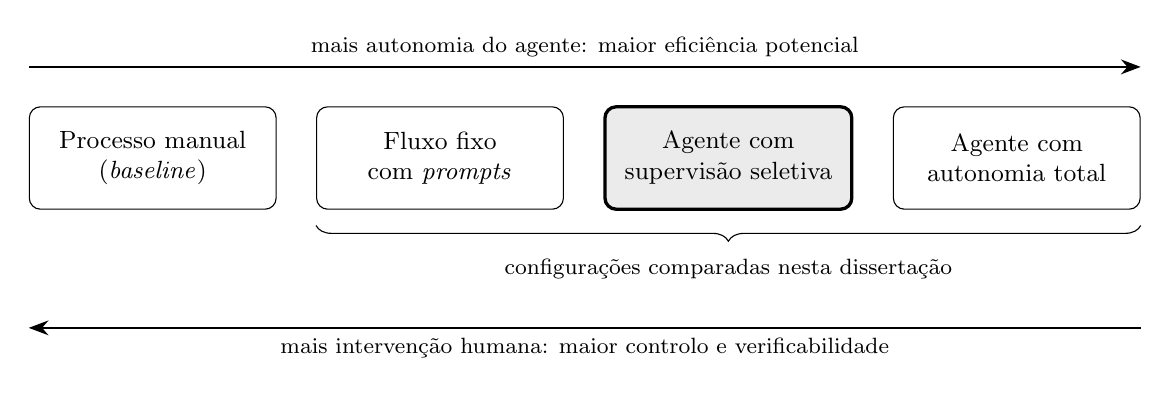
\begin{tikzpicture}[
      node distance=5mm,
      etapa/.style={draw, rounded corners, align=center, minimum height=13mm, text width=29mm, font=\small},
      arr/.style={-{Stealth[length=2.5mm]}, thick}
    ]
    \node[etapa] (man) {Processo manual\\(\textit{baseline})};
    \node[etapa, right=of man] (fix) {Fluxo fixo\\com \textit{prompts}};
    \node[etapa, right=of fix, fill=black!8, very thick] (sel) {Agente com\\supervisão seletiva};
    \node[etapa, right=of sel] (aut) {Agente com\\autonomia total};

    \draw[arr] ([yshift=5mm]man.north west) -- node[above, font=\footnotesize]{mais autonomia do agente: maior eficiência potencial} ([yshift=5mm]aut.north east);
    \draw[decorate, decoration={brace, mirror, amplitude=2mm}] ([yshift=-2mm]fix.south west) -- node[below=3mm, font=\footnotesize]{configurações comparadas nesta dissertação} ([yshift=-2mm]aut.south east);
    \draw[arr] ([yshift=-15mm]aut.south east) -- node[below, font=\footnotesize]{mais intervenção humana: maior controlo e verificabilidade} ([yshift=-15mm]man.south west);
  \end{tikzpicture}
  \caption[Espetro entre intervenção humana e autonomia do agente]{Espetro entre intervenção humana e autonomia do agente. Os extremos favorecem um objetivo à custa do outro. A configuração destacada concentra a supervisão humana nas ações críticas, de acordo com um modelo de autonomia, e é a que esta dissertação procura conceber e validar.}
  \label{fig:espetro_autonomia}
\end{figure}

A estas dificuldades junta-se uma restrição concreta do contexto. A confidencialidade dos dados da empresa pode limitar a informação que é possível usar durante o desenvolvimento e os ensaios, bem como o que é possível publicar nesta dissertação. Sempre que necessário, serão usados dados anonimizados ou sintéticos, que permitem reproduzir as características relevantes dos processos sem expor informação sensível.

%----------------------------------------------------------------------------------------
\section{Questões de Investigação}
\label{sec:introducao_questoes}
%----------------------------------------------------------------------------------------

O problema descrito conduz à questão de investigação principal desta dissertação:

\begin{description}
  \item[QP.] Como conceber agentes baseados em \glspl{llm} que automatizem processos internos de \gls{id} em saúde digital, mantendo supervisão humana e rastreabilidade, com ganhos mensuráveis de eficiência sem perda de qualidade nem de confiança por parte da equipa?
\end{description}

A questão principal é de natureza construtiva: a resposta toma a forma de um artefacto, composto por um modelo de autonomia e por um protótipo que o concretiza, e das orientações que dele se extraem. Para que essa resposta possa ser avaliada, é complementada por uma questão secundária, de natureza empírica:

\begin{description}
  \item[QS.] Qual é o impacto dessa automação na eficiência dos processos, na qualidade dos resultados e na aceitação por parte da equipa?
\end{description}

A questão secundária decompõe-se em três dimensões, que correspondem aos três eixos de avaliação descritos na Secção~\ref{sec:introducao_abordagem}: a eficiência, medida pelo tempo total necessário para concluir cada processo; a qualidade, medida pela correção e completude dos resultados e pela capacidade de detetar erros; e a aceitação, medida pela usabilidade percebida e pela utilidade atribuída pela equipa. Estas questões distinguem-se das questões da revisão sistemática da literatura (Capítulo~\ref{chap:estado_arte}), que se destinam a caracterizar o conhecimento existente e não a orientar a conceção da solução.

%----------------------------------------------------------------------------------------
\section{Objetivos}
\label{sec:introducao_objetivos}
%----------------------------------------------------------------------------------------

O objetivo geral desta dissertação é conceber, implementar e avaliar agentes baseados em \glspl{llm} com supervisão humana para processos internos de \gls{id} da VirtualCare, e extrair desse trabalho orientações replicáveis para a integração deste tipo de agentes em fluxos de trabalho organizacionais sensíveis. Este objetivo concretiza-se nos sete objetivos específicos da Tabela~\ref{tab:objetivos}, cada um associado a um critério que permite verificar o seu cumprimento.

\begin{table}[htbp]
  \centering
  \caption{Objetivos específicos e respetivos critérios de cumprimento}
  \label{tab:objetivos}
  \small
  \begin{tabularx}{\textwidth}{@{}l >{\raggedright\arraybackslash}X >{\raggedright\arraybackslash}X c@{}}
    \toprule
    & \textbf{Objetivo} & \textbf{Critério de cumprimento} & \textbf{Cap.} \\
    \midrule
    O1 & Mapear processos de \gls{id} candidatos e selecionar os que serão automatizados & 2 a 3 processos mapeados e 2 selecionados com critérios explícitos (frequência, esforço, risco e qualidade) & \ref{chap:metodologia} \\
    \addlinespace
    O2 & Definir um modelo de autonomia para cada processo selecionado & Todas as ações classificadas como autónomas, sujeitas a aprovação ou proibidas, com justificação & \ref{chap:concecao} \\
    \addlinespace
    O3 & Implementar um protótipo que concretize o modelo de autonomia & Nenhuma ação irreversível executada sem aprovação; 100\% das ações registadas em \textit{log} de auditoria & \ref{chap:implementacao} \\
    \addlinespace
    O4 & Melhorar a eficiência dos processos & Redução de pelo menos 30\% do tempo total (geração e revisão) face ao processo manual & \ref{chap:avaliacao} \\
    \addlinespace
    O5 & Manter a qualidade dos resultados & Pelo menos 85\% de correção e completude; pelo menos 80\% dos erros injetados detetados & \ref{chap:avaliacao} \\
    \addlinespace
    O6 & Obter a aceitação da equipa & Pontuação \gls{sus} igual ou superior a 68; utilidade percebida igual ou superior a 4 em 5 & \ref{chap:avaliacao} \\
    \addlinespace
    O7 & Sistematizar orientações replicáveis & Orientações documentadas e validadas com a empresa & \ref{chap:conclusoes} \\
    \bottomrule
  \end{tabularx}
\end{table}

Os objetivos O1 a O3 dizem respeito à construção do artefacto e os objetivos O4 a O6 à sua avaliação; o objetivo O7 sintetiza o conhecimento produzido. Algumas metas merecem uma explicação adicional.

A meta de eficiência (O4) refere-se ao \emph{tempo total} do processo, que inclui não só a geração do resultado pelo agente, mas também o tempo que a equipa gasta a rever e a corrigir esse resultado. Esta opção é deliberada: uma solução que gere documentos em segundos, mas que obrigue a uma revisão mais demorada do que a escrita manual, não representa um ganho real. Pela mesma razão, a meta de qualidade (O5) combina duas medidas. A correção e a completude avaliam os resultados produzidos face a uma grelha definida com a equipa. A taxa de deteção de erros injetados avalia a eficácia da supervisão: são introduzidos deliberadamente erros conhecidos nos resultados intermédios e mede-se a proporção que é identificada antes de produzir efeitos, pelas salvaguardas automáticas ou pelos revisores humanos. Esta segunda medida responde diretamente ao risco de viés de automação discutido na Secção~\ref{sec:introducao_problema}.

A aceitação (O6) é medida com dois instrumentos. O \gls{sus} é um questionário padronizado de dez itens que produz uma pontuação de usabilidade entre 0 e 100 \parencite{brooke1996sus}; o valor de 68 corresponde aproximadamente à média observada em centenas de estudos e é habitualmente usado como limiar de usabilidade aceitável \parencite{bangor2009determining,sauro2011practical}. A utilidade percebida, um dos construtos centrais do modelo de aceitação de tecnologia de \textcite{davis1989perceived}, é medida numa escala de 1 a 5. Os dois instrumentos são apresentados em pormenor no Capítulo~\ref{chap:fundamentos}.

As metas quantitativas foram definidas na proposta desta dissertação com base na literatura e nas expectativas iniciais da empresa. Poderão ser ajustadas depois do levantamento dos processos, caso este revele características que as tornem desadequadas; qualquer ajuste será justificado no Capítulo~\ref{chap:metodologia}, antes do início dos ensaios.
% TODO: validar as metas de O4 a O6 com a VirtualCare e com os orientadores antes de as fixar.

%----------------------------------------------------------------------------------------
\section{Abordagem}
\label{sec:introducao_abordagem}
%----------------------------------------------------------------------------------------

O trabalho segue a metodologia \gls{dsr}, que enquadra a investigação como a construção e avaliação de um artefacto concebido para resolver um problema prático relevante \parencite{hevner2004design}. A escolha justifica-se pela natureza da questão principal: o que se pretende não é apenas descrever ou explicar um fenómeno, mas conceber uma solução e demonstrar, com evidência, que ela cumpre os objetivos definidos. Neste trabalho, o artefacto é composto pelo modelo de autonomia e pelo protótipo de agentes que o concretiza. O processo segue as seis atividades propostas por \textcite{peffers2007design}, cuja concretização neste trabalho se resume na Tabela~\ref{tab:dsr_atividades}.

\begin{table}[htbp]
  \centering
  \caption{Concretização das atividades da \gls{dsr} neste trabalho}
  \label{tab:dsr_atividades}
  \small
  \begin{tabularx}{\textwidth}{@{}>{\raggedright\arraybackslash}p{3.6cm} >{\raggedright\arraybackslash}X c@{}}
    \toprule
    \textbf{Atividade} & \textbf{Concretização} & \textbf{Cap.} \\
    \midrule
    Identificação do problema e motivação & Contexto da VirtualCare, revisão da literatura e levantamento dos processos por entrevistas à equipa de \gls{id} & \ref{chap:introducao}, \ref{chap:estado_arte}, \ref{chap:metodologia} \\
    \addlinespace
    Definição dos objetivos da solução & Objetivos O1 a O7 e requisitos derivados do levantamento & \ref{chap:introducao}, \ref{chap:metodologia} \\
    \addlinespace
    Conceção e desenvolvimento & Modelo de autonomia, arquitetura dos agentes e protótipo para os dois processos selecionados & \ref{chap:concecao}, \ref{chap:implementacao} \\
    \addlinespace
    Demonstração & Utilização do protótipo pela equipa em casos reais ou representativos dos processos & \ref{chap:implementacao} \\
    \addlinespace
    Avaliação & Ensaios comparativos nos eixos de eficiência, qualidade e aceitação & \ref{chap:avaliacao} \\
    \addlinespace
    Comunicação & Esta dissertação e as orientações entregues à empresa & \ref{chap:conclusoes} \\
    \bottomrule
  \end{tabularx}
\end{table}

Em termos práticos, o trabalho desenvolve-se em quatro passos. Primeiro, é feito o levantamento dos processos candidatos através de entrevistas à equipa de \gls{id}, de modo a descrever cada processo, estimar o esforço que exige e identificar os seus riscos; daqui resulta a seleção dos dois processos a automatizar (O1). Segundo, é desenhado o modelo de autonomia de cada processo, que classifica cada ação possível do agente numa de três categorias: autónoma, sujeita a aprovação ou proibida (O2). É também desenhada a arquitetura dos agentes, incluindo as ferramentas a que têm acesso, a componente de \gls{rag} e o mecanismo de registo. Terceiro, é implementado um protótipo funcional para os dois processos (O3). Quarto, são realizados ensaios comparativos com a equipa (O4 a O6).

A Figura~\ref{fig:visao_geral} apresenta a visão geral da solução que resulta destes passos. A equipa formula um pedido e o agente, apoiado na documentação da empresa através de \gls{rag}, planeia o trabalho e propõe as ações necessárias. Nenhuma ação é executada diretamente: cada uma passa primeiro pelo modelo de autonomia, que a encaminha conforme a sua classe. As ações autónomas são executadas de imediato; as ações sujeitas a aprovação aguardam a decisão de um revisor humano; as ações proibidas são bloqueadas. Todas as ações e decisões, incluindo as aprovações e as rejeições, ficam guardadas no registo de auditoria, o que permite reconstituir, a qualquer momento, o que o agente fez, com base em que informação e com a autorização de quem.

\begin{figure}[htbp]
  \centering
  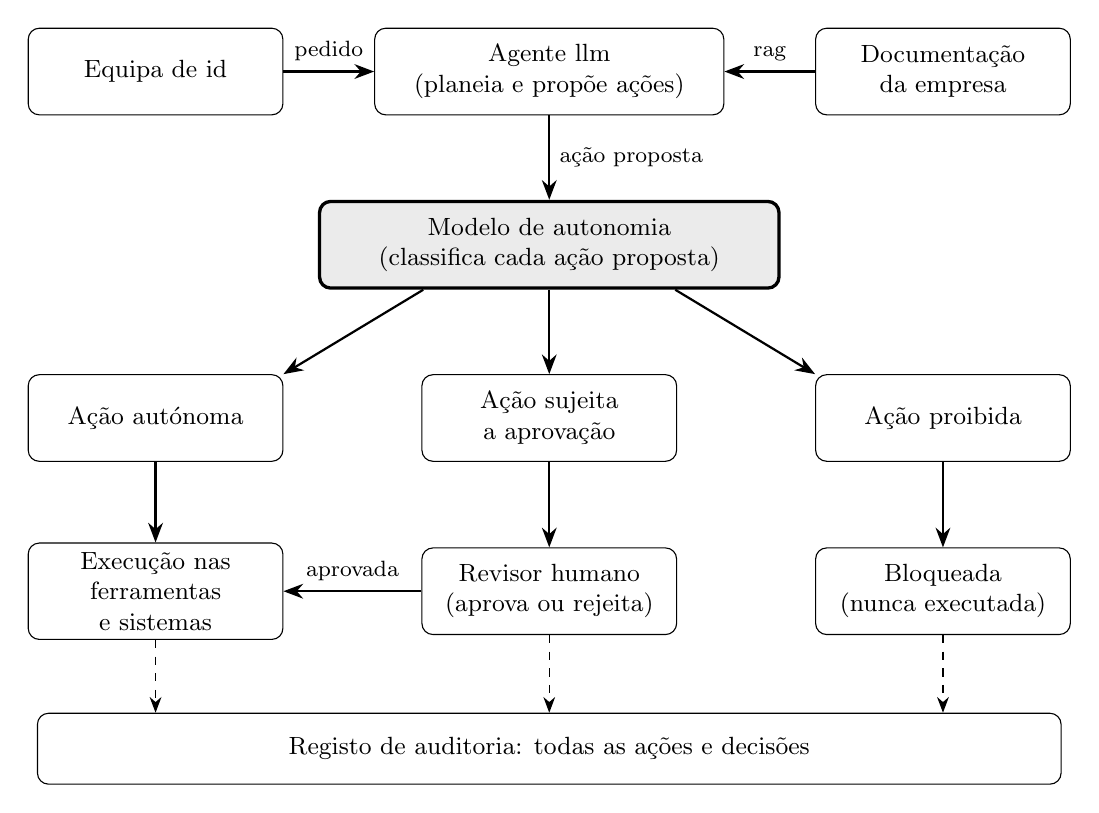
\begin{tikzpicture}[
      box/.style={draw, rounded corners, align=center, minimum height=11mm, text width=30mm, font=\small},
      gate/.style={draw, rounded corners, very thick, fill=black!8, align=center, minimum height=11mm, text width=56mm, font=\small},
      arr/.style={-{Stealth[length=2.5mm]}, thick},
      log/.style={-{Stealth[length=2mm]}, dashed},
      lbl/.style={font=\footnotesize}
    ]
    \node[box] (team) at (0,0) {Equipa de \gls{id}};
    \node[box, text width=42mm] (agent) at (5,0) {Agente \gls{llm}\\(planeia e propõe ações)};
    \node[box] (docs) at (10,0) {Documentação\\da empresa};
    \node[gate] (model) at (5,-2.2) {Modelo de autonomia\\(classifica cada ação proposta)};
    \node[box] (auto) at (0,-4.4) {Ação autónoma};
    \node[box] (appr) at (5,-4.4) {Ação sujeita\\a aprovação};
    \node[box] (forb) at (10,-4.4) {Ação proibida};
    \node[box] (exec) at (0,-6.6) {Execução nas\\ferramentas e sistemas};
    \node[box] (human) at (5,-6.6) {Revisor humano\\(aprova ou rejeita)};
    \node[box] (block) at (10,-6.6) {Bloqueada\\(nunca executada)};
    \node[draw, rounded corners, align=center, minimum height=9mm, minimum width=130mm, font=\small] (audit) at (5,-8.6) {Registo de auditoria: todas as ações e decisões};

    \draw[arr] (team) -- node[above, lbl]{pedido} (agent);
    \draw[arr] (docs) -- node[above, lbl]{\gls{rag}} (agent);
    \draw[arr] (agent) -- node[right, lbl]{ação proposta} (model);
    \draw[arr] (model.south) ++(-1.6,0) -- (auto.north east);
    \draw[arr] (model) -- (appr);
    \draw[arr] (model.south) ++(1.6,0) -- (forb.north west);
    \draw[arr] (auto) -- (exec);
    \draw[arr] (appr) -- (human);
    \draw[arr] (forb) -- (block);
    \draw[arr] (human) -- node[above, lbl]{aprovada} (exec);
    \draw[log] (exec) -- (exec |- audit.north);
    \draw[log] (human) -- (audit);
    \draw[log] (block) -- (block |- audit.north);
  \end{tikzpicture}
  \caption[Visão geral da solução proposta]{Visão geral da solução proposta. O agente apenas propõe ações; o modelo de autonomia decide se cada uma é executada de imediato, submetida a um revisor humano ou bloqueada. Todas as ações e decisões ficam no registo de auditoria.}
  \label{fig:visao_geral}
\end{figure}

A avaliação assenta em três eixos, que respondem às três dimensões da questão secundária:

\begin{itemize}
  \item \textbf{Eficiência:} tempo total de execução de cada processo, incluindo geração e revisão, comparado com o do processo manual.
  \item \textbf{Qualidade:} correção e completude dos resultados, avaliadas com uma grelha definida em conjunto com a equipa, e taxa de deteção de erros injetados.
  \item \textbf{Aceitação:} questionário \gls{sus} e inquérito sobre a utilidade percebida e a confiança nos resultados.
\end{itemize}

Para perceber que fatores explicam os resultados, e não apenas se a solução final funciona, são comparadas pelo menos três configurações com diferentes graus de autonomia: um fluxo fixo baseado em \textit{prompts}, em que a sequência de passos é definida pelo programador e o modelo não decide que ações executar; um agente com ferramentas e \gls{rag}, que decide autonomamente a sequência de ações; e variantes intermédias com diferentes níveis de supervisão humana, obtidas aplicando o modelo de autonomia. Estas configurações correspondem a posições distintas do espetro da Figura~\ref{fig:espetro_autonomia}. O termo de comparação (\textit{baseline}) é o processo manual atualmente seguido pela equipa. Esta comparação permite separar o efeito da tecnologia (o \gls{llm} e o \gls{rag}) do efeito do grau de autonomia concedido, que é a variável central desta dissertação.

O trabalho está organizado em duas fases. Na primeira, correspondente ao primeiro semestre, realizam-se a revisão do estado da arte, o levantamento dos processos e o desenho do modelo de autonomia e da arquitetura. Na segunda, correspondente ao segundo semestre, realizam-se a implementação do protótipo, os ensaios com a equipa e a conclusão da escrita da dissertação.

Com esta abordagem, espera-se que o trabalho produza as seguintes contribuições:

\begin{enumerate}
  \item um \textbf{modelo de autonomia} que classifica as ações de um agente em autónomas, sujeitas a aprovação ou proibidas, com critérios explícitos para essa classificação;
  \item um \textbf{protótipo} de agentes baseados em \glspl{llm} para dois processos reais de \gls{id}, com supervisão humana nos pontos críticos e registo de auditoria completo;
  \item \textbf{evidência empírica} sobre a eficiência e a qualidade obtidas com diferentes níveis de autonomia, num contexto organizacional real de saúde digital;
  \item um conjunto de \textbf{orientações replicáveis} para a integração de agentes baseados em \glspl{llm} em fluxos de trabalho organizacionais sensíveis, validadas com a empresa.
\end{enumerate}

%----------------------------------------------------------------------------------------
\section{Estrutura do Documento}
\label{sec:introducao_estrutura}
%----------------------------------------------------------------------------------------

Além desta introdução, o documento está organizado em mais sete capítulos.

O Capítulo~\ref{chap:fundamentos}, \textit{Fundamentos Teóricos}, apresenta os conceitos em que o trabalho assenta: os \glspl{llm}, os agentes e o uso de ferramentas, o \gls{rag}, os modelos de autonomia e supervisão humana, os riscos associados, a rastreabilidade, as métricas de avaliação e o enquadramento regulatório europeu.

O Capítulo~\ref{chap:estado_arte}, \textit{Estado da Arte}, descreve a revisão sistemática da literatura, conduzida segundo as diretrizes de \textcite{kitchenham2007guidelines} e reportada segundo o \gls{prisma} \parencite{page2021prisma}, e identifica as lacunas a que esta dissertação procura responder.

O Capítulo~\ref{chap:metodologia}, \textit{Metodologia e Análise do Problema}, detalha a aplicação da \gls{dsr}, apresenta o levantamento dos processos na VirtualCare, os requisitos identificados e os critérios que justificam a seleção dos dois processos a automatizar.

O Capítulo~\ref{chap:concecao}, \textit{Conceção da Solução}, apresenta o modelo de autonomia, a arquitetura dos agentes e os mecanismos de deteção de erros, salvaguarda e rastreabilidade.

O Capítulo~\ref{chap:implementacao}, \textit{Implementação}, descreve o protótipo desenvolvido e a sua integração nos processos selecionados.

O Capítulo~\ref{chap:avaliacao}, \textit{Avaliação}, define o protocolo de avaliação e as métricas usadas, descreve as configurações comparadas e o \textit{baseline}, e apresenta e discute os resultados obtidos.

Por fim, o Capítulo~\ref{chap:conclusoes}, \textit{Conclusões e Trabalho Futuro}, responde às questões de investigação, sintetiza as contribuições e as orientações produzidas, discute as limitações do trabalho e aponta direções para trabalho futuro.

% Capítulo 2
\chapter{Fundamentos Teóricos}
\label{chap:fundamentos}
% TODO: fundamentos teóricos

% Capítulo 3
\chapter{Estado da Arte}
\label{chap:estado_arte}

% TODO: parágrafo de introdução. Este capítulo analisa, através de uma revisão
% sistemática da literatura, como os conceitos do Capítulo~\ref{chap:fundamentos}
% têm sido combinados em trabalhos recentes.

\section{Metodologia da Revisão}
\label{sec:estado_arte_metodologia}
% TODO: revisão sistemática seguindo Kitchenham e Charters (2007) e o fluxo PRISMA 2020 (Page et al., 2021).
% Revisor único: documentar as adaptações ao processo.

\subsection*{Questões de Investigação}
% TODO: tabela com as questões. Proposta inicial (a validar com a orientadora):
%  QI1 - Como têm sido aplicados agentes baseados em LLM na automação de processos
%        de trabalho de conhecimento e de documentação em contexto organizacional?
%  QI2 - Que mecanismos de supervisão humana e de controlo de autonomia têm sido
%        propostos para agentes baseados em LLM?
%  QI3 - Que mecanismos de rastreabilidade e de deteção de erros são usados nestes sistemas?
%  QI4 - Como são avaliados estes sistemas em termos de eficiência, qualidade e aceitação?

\subsection*{Estratégia de Pesquisa}
% TODO: bases de dados (Scopus, IEEE Xplore, ACM DL, Web of Science), string de pesquisa, data da pesquisa

\subsection*{Critérios de Inclusão e Exclusão}
% TODO: tabelas de critérios (CI1..., CE1...)

\subsection*{Seleção dos Estudos}
% TODO: diagrama PRISMA e avaliação de qualidade

\section{Revisão da Literatura}
\label{sec:estado_arte_revisao}
% TODO: uma subsecção por questão de investigação, cada uma terminando com uma síntese

\section{Lacunas Identificadas}
\label{sec:estado_arte_lacunas}
% TODO: síntese e lacunas que justificam o trabalho

% Capítulo 4
\chapter{Metodologia e Análise do Problema}
\label{chap:metodologia}

\section{Design Science Research}
\label{sec:metodologia_dsr}
% TODO: aplicação da metodologia

\section{Levantamento de Processos na VirtualCare}
\label{sec:metodologia_levantamento}
% TODO: resultados do levantamento

\section{Requisitos}
\label{sec:metodologia_requisitos}
% TODO: requisitos identificados

\section{Seleção dos Processos}
\label{sec:metodologia_selecao}
% TODO: critérios e processos selecionados

% Capítulo 5
\chapter{Conceção da Solução}
\label{chap:concecao}

\section{Modelo de Autonomia}
\label{sec:concecao_autonomia}
% TODO: modelo de autonomia

\section{Arquitetura dos Agentes}
\label{sec:concecao_arquitetura}
% TODO: arquitetura

\section{Deteção de Erros e Salvaguardas}
\label{sec:concecao_salvaguardas}
% TODO: deteção de erros e salvaguardas

\section{Rastreabilidade}
\label{sec:concecao_rastreabilidade}
% TODO: mecanismos de rastreabilidade

% Capítulo 6
\chapter{Avaliação}
\label{chap:avaliacao}

\section{Protocolo e Métricas}
\label{sec:avaliacao_protocolo}
% TODO: eficiência, qualidade, aceitação (SUS)

\section{Configurações Comparadas e Baseline}
\label{sec:avaliacao_configuracoes}
% TODO: configurações e baseline

\section{Resultados}
\label{sec:avaliacao_resultados}
% TODO: resultados

\section{Discussão}
\label{sec:avaliacao_discussao}
% TODO: discussão

% Capítulo 7
\chapter{Conclusões e Trabalho Futuro}
\label{chap:conclusoes}
% TODO: conclusões e trabalho futuro

% Capítulo 8
\chapter{Conclusões e Trabalho Futuro}
\label{chap:conclusoes}
% TODO: conclusões e trabalho futuro


%----------------------------------------------------------------------------------------
%	BIBLIOGRAPHY
%----------------------------------------------------------------------------------------

\printbibliography[heading=bibintoc]

%----------------------------------------------------------------------------------------
%	APPENDICES
%----------------------------------------------------------------------------------------

\begin{appendices}

% Apêndice A
\chapter{Material Suplementar} % TODO: título provisório
\label{app:material_suplementar}


\end{appendices}

\end{document}
